\chapter{Business Model for the Microsoft Kinect Based Exergame}
In this chapter we will use the information assembled in the previous chapters to  make an analysis of the business opportunities of the exergame. We will provide a detailed description of a business model that describes how the game should be created and delivered, and how it can create value. As a framework for this description, we will use Osterwalder's Business Model Ontology, as described in Chapter 5. \\ \\ 
In this chapter we will describe the potential of Cyberlab's exergame through all of the nine building blocks.  

\section{Product}
A product covers all aspects of what a company offers to its customers. The product is composed of value propositions, which are services and values offered to the customer. Cyberlab’s product is an exergame which is meant to be used by physiotherapists as a tool for exercising and rehabilitation for elderly. The focus of the exergame is to improve strength and balance in elderly to prevent fall and injuries. By using the exergame, this can be done in a more amusing and motivating way. The game will have one general workout version for training and one customized version used in rehabilitation. The exergame will be developed for the Microsoft Kinect sensor for Windows, which tracks body movement without the use of any controllers. This makes it convenient to use for elderly, as it allows them to only focus on the tasks provided by the game. The exergame will be used in physiotherapy clinics, where physiotherapists can set up customized programs and guide their patients through the exercise. The Microsoft Kinect sensor provides useful feedback to the physiotherapists when it comes to measuring the execution of the exercises and their patients progression. 
\subsection{Value Proposition}
The exergame's value proposition can be described as: \\ \\
\emph{A tool with the ability to customize an exercise program and to offer an alternative, fun and motivating training method while at the same time ease the workload of the physiotherapist}\\ \\
Value propositions refer to the value a company offers to a specific customer segment. One value this product provides is the possibility to offer an alternative, fun and motivating training method. The exergame is meant to be used as a supplement in training programs or as an exercise motivator. A good motivator is a social aspect, which is highly important for elderly, and that there exist games for different interests. The game can also be used as a tool for physiotherapists to make it easier to customize training programs for their patients. Every patient is different, with individual problems and needs, and it is therefore necessary to provide personalized exercise program for each patient. An important value the product has to serve is that the exergame can set up training programs and be more motivating than a physiotherapist can. 
\section{Customer Interface}
In this section we will describe how Cyberlab can create value for the customers. In particular we will discuss who the customers are, how to reach out to them and what kind of customer relationships should be maintained after the sale. 
\subsection{Customer Segments}
In general, a company generates value for a specific customer segment. To define the right segment for Cyberlab, we studied different groups of people; elderly who are the end user of the game, and several entities related to elderly, like training groups, community centres, and physiotherapists.\\ \\ 
\emph{Elderly:}\\ 
The end user of the exergame are the older population and they are therefore considered as a possible customer segment. The idea would be to sell the game directly to elderly so they can use this exergame at home. The fair of falling makes many elderly afraid of walking outside their own house. Therefore, it would be appealing for them to have the possibility to exercise at home. In order to become physically stronger, there is a need for a supplement to the weekly physiotherapy appointments or training group sessions. Regular workout at home will strengthen muscles and increase balance.  This may contribute to prevention of falling and increased self confidence. The connection this game has to fun and entertainment in stead of "workout" is a motivating factor to exercise more. A social factor is also included, which is important for elderly who spends a lot of time alone. \\ \\
\emph{Training groups:}\\ 
There exist several training groups focusing on elderly who can be a possible customer segment for Cyberlab. Here, elderly pay a small fee to join a training group, which is fun, social and more motivating than exercising alone. These training groups are engaged by the government, physiotherapy clinics, organizations and individuals. During these workout sessions this exergame can be used as a supplement or a different alternative to ordinary exercise. Playing the exercise together with other elderly makes the game social and entertaining. \\ \\
\emph{Community centres:} \\
We evaluated community centres for elderly as a possible customer segment. These centres will buy the product and all the equipment needed from Cyberlab and install it in their own environment. With this game they can provide the elderly with an alternative activity compared to chess, card play or taking a walk. One possibility for the community centres is to rent out the game to their patients, so the patients can use the equipment for a certain amount of time, alone or in a group. \\ \\
\emph{Physiotherapists:} \\
Physiotherapists have very close relationship to elderly, and their goal is to help them decrease the risk of falling by using mobility techniques to improve balance and physical strength. Physiotherapists are also a group with a certain authority appearance, which makes them trustworthy. Physiotherapists can buy this product, install it in their environment and use it as a tool for training, both in an individual therapy session and in a training group. \\ \\
After composing, studying and discussing business models for each possible customer segment, we recommend Cyberlab to focus on physiotherapy clinics as customers. More precisely,  we will recommend to start with public clinics and private clinics with contribution from the government. The goal of their work fits well with the purpose of Cyberlab's exergame, and the authority they have is very valuable when trying to get elderly to adapt the new technology this game provides. The recommended physiotherapy clinics have access to a wide customer base consisting of elderly. It is also important to emphasis the importance of the new reform "Samhandlingsreformen", which encourage the use of welfare technology where possible. This suggest that there is a place for an exergame in the health sector.  The economy in this entity is controlled by the government. With the support from the new reform, we believe there should be no economical issues around investing in a game like this. 

\subsection{Channels}
In this subsection we will describes how Cyberlab should deliver and market their value propositions to their customer segment. We will describe this by going through the five channel phases.\\ \\
\begin{figure}
\label{fig:Channels}
\begin{center}
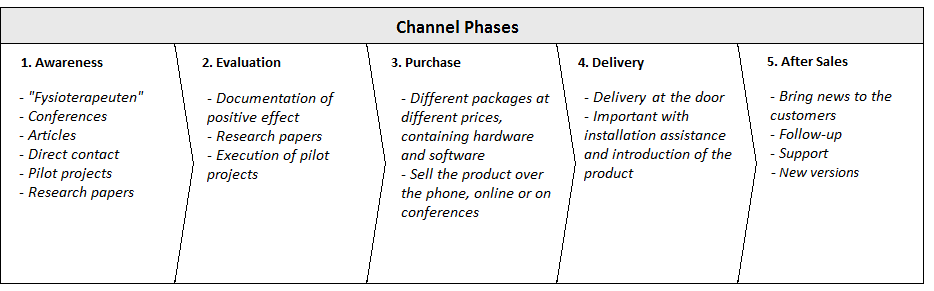
\includegraphics[angle=90,scale=0.7]{channels}
\caption[Channels]{The 5 Channel Phases [modified from \cite{osterwalder}\cite{osterwalderthesis}]}
\end{center}
\end{figure}
\emph{Awareness:} \\ 
We will look into some activities Cyberlab should perform to raise awareness about their product and how they can get their customers attention. "Fysioterapeuten" is a magazine targeting physiotherapists in Norway. This magazine is published by \ac{nff} and distributed to the whole country. "Fysioterapeuten" contains mostly scientific papers, and the idea is that this magazine shall contribute to evolvement of the physiotherapy profession. This magazine is read by 9 000 physiotherapists around the country, and articles printed here are seen as scientific and are therefore taken seriously. Cyberlab should use "Fysioterapeuten" as a medium to promote the exergame by printing an article or an ad. Printing research papers and articles about the exergame in other credible magazines or newspapers is also a way to get physiotherapists attention. \\ \\
Another solution for Cyberlab is to promote their product by taking direct contact with the customer segment. This could be done by joining conferences related to subjects like e.g. welfare technology or by visiting physiotherapy clinics. Cyberlab will then get the opportunity to present the product and show direct interest in establishing a customer relationship. An example of a highly relevant conference for Cyberlab to attend is "Velferdsteknologikonferansen" \cite{conference}. This is a conference that has been held in Trondheim three times, and is describes as a conference for people that are interested in welfare technology and "Samhandlingsreformen". Physiotherapists see it as very relevant to try a product for an amount of time before they decide to buy. Cyberlab can raise awareness of the product by announcing that they need participants for a pilot project. Awareness can also arise from an already ongoing pilot project. \\ \\
\emph{Evaluation:}\\
Physiotherapists points out two very important aspects in evaluating a product. These two are; documented effect of the product and own experience by testing the product. If a physiotherapist should even think about trying the product, it is necessary to provide research papers and statistics that show positive effect on the use of this kind of game. Documentation will give them a security in the choice of buying the product. Other physiotherapists providing positive feedback after trying the game also contributes to this security. We suggest that Cyberlab should start pilot projects at one or more physiotherapy clinics, as this is a good way to be evaluated. A pilot project will provide the physiotherapists with the possibility to test, experience and evaluate the product themselves for a period of time. The evaluation received from the pilot projects should be used as documentation for the product.\\ \\
\emph{Purchase:} \\
Most physiotherapists have already established connections with suppliers. Ordering and buying products are usually done online, but it can also be by phone or when interesting products are discovered on conferences. Going to the store to buy products is very unusual. To play this game there are software and hardware needed, like Microsoft Kinect sensor and the exergame. It is unreasonable to think that a physiotherapist already owns a Kinect sensor, so the best strategy for Cyberlab is to sell packages containing both hardware and software. Packages should include various agreements with appropriate pricing. \\ \\
\emph{Delivery:}\\
When buying a new product, especially technical products, there is a need for introduction to the product and maybe also installation assistance. Feedback from interviews with physiotherapists shows the huge importance of start-up help. With busy days at work, physiotherapists do not have time to pick up deliveries at the postal office, or to setup and learn new products all by themselves. Buying, receiving, installing and learning should not be difficult or time consuming. \\ \\
From the interviews conducted we found that it was desirable with installation and introduction help when buying technical equipment, so the product should be delivered at the door, by someone who can install the product and teach the physiotherapists how to use it. However, this is a complicated task for Cyberlab if we look at every physiotherapy clinic as their customer segment. It is not realistic that one representative from Cyberlab will travel to the other side of the country as soon as a clinic order the game. Therefore, we will not take this into consideration in this assignment, but there is still an issue to take into account.\\ \\
\emph{After sales:}\\
When taking a new product in to use, it is important for physiotherapist to have the possibility to come with feedback. Therefore, Cyberlab should have some kind of support that can take these feedbacks into consideration. Feedbacks can be comments on direct errors or directions on how to make the exergame more suitable for its use. Cyberlab should follow their customer in the process of learning, and they should inform them of new features and improvements.  
\subsection{Customer Relationships}
Customer relationship is an important part of the customer experience, and it describes what kind of relationship the company establishes with the customers. Support, follow-up and feedback handling are some aspects in establishing customer relationship. Cyberlab has to be available when the customers have problems and need help. When using a new product one may discover errors or find the product not suitable for its use, so many physiotherapists have an eager to provide feedback on this. Cyberlab should handle these feedbacks and fix errors as soon as possible and take comments on improvements into consideration. Using feedback to make a better product shows customers that Cyberlab takes their comments seriously.  In addition, the customers will hopefully get a more suitable product. The maintenance of a direct and personal contact with the customer shows interest in the use and the experience of the product. All this can contribute to a good customer relationship. Cyberlab should also give their customers a heads ups on updates, new features or products.
\section{Infrastructure Management}
This section is about how Cyberlab creates value. What resources needed and what activities that have to be preformed are described here, as well as if they will get them in-house or from a partner. 

\subsection{Key Resources}

In this section we will describe all the resources needed to make the business model work. The resources are divided into 4 different types, described in table \ref{tab:Resources}.
\newpage

\begin{table}
\centering
    \begin{tabular}{|l|l|}
        \hline
       \textbf{Type of Resource} & \textbf{Resource}  \\ \hline
       \emph{Intellectual} & Insight and experience with fall problematic \\ & in elderly \\ \cline{2-2}
        & Programming skills \\ \cline{2-2}
	 	& Creativity \\ \hline
	   \emph{Physical} & Premises \\ \cline{2-2}
	   	& Equipments, i.e. desks and computers  \\ \cline{2-2}
	   	& Microsoft Kinect sensor \\ \cline{2-2}
	   	& Windows machines \\ \cline{2-2}
	   	& Projector and screen \\ \cline{2-2}
	   	& Working Environment, Kinect for Windows SDK \\ \cline{2-2}
	   	& Internet Connections \\ \hline
	   \emph{Human} & System Developers, i.e. programmers and \\ & interaction designers \\ \cline{2-2}
	   	& Administration, i.e. marketers, customer related \\ &tasks \\ \cline{2-2}
	   	& Support Person(s) \\ \hline
	   \emph{Financial} & The European Union \\
        \hline
    \end{tabular}
    \caption[Resources]{Different types of resources}
    \label{tab:Resources}
\end{table} 
\emph{Intellectual} \\ The developer team needs insight and knowledge about different exercises that will strengthen muscles and improve balance in elderly. Cyberlab is provided with research information from other entities in this project, so their job will be to process this information. When they have enough knowledge to form the foundation of an exercise program, they can start to get creative. Creativity is needed to make the game entertaining and easy to understand and conduct. In addition, good programming competencies are needed to develop the game. To make it as cost-efficient as possible, an experienced team should be put together. \\ \\
\emph{Physical} \\ To be able to conduct this project, the team needs premises with everything that comes with it, like desks, chairs, computer, internet connection, lights etc. Cyberlab is an already established business, so we can assume they already have these premises and equipment established, and that this will not provide any additional costs. For this project, they will need specific hardware. The hardware consists of the Kinect sensor, a Windows machine, a server for storing and running the game and a projector and screen for testing purposes. In addition they will need the Kinect for Windows SDK to be able to develop a game for this platform.\\ \\
\emph{Human} \\ Programming skills and creativity are already described above as intellectual resources. So they will need system developers and interaction designers. An administration is needed for marketing, customer related tasks and resource management. When the game is finished it needs to be operated and maintained. These tasks can be done by one or more of the system developers. \\ \\
\emph{Finance} \\ This project is financed by the European Union. However, we will not take this into account when looking at the financial aspects of this game. The reason for this is that Cyberlab...

\subsection{Key Activities}
The game can be described as a Value Chain, which means transforming inputs into a final product. From the knowledge and experience Cyberlab has acquired they want to make a product as good, cost efficient, and price-competitive so that their customers would choose their product instead of a product with similar value. A description of the different stages in the value chain is depicted in figure \ref{fig:ValueChainCase}. The development of the game should be test-driven, meaning that they will test the product both on the end-users and the customer segment during the development, and adapt the game based on the experiences acquired during the testing. Activities that need to be done include research processing, development, testing, maintenance and updates, support, marketing and administrative tasks, shown in table \ref{tab:activities}. 


\begin{figure}
\begin{center}
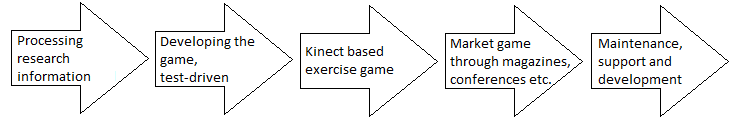
\includegraphics[scale=0.7]{valuechaincase}
\caption[Value Chain for the Kinect Based Exergame]{Value chain for the Kinect based exergame [modified from \cite{osterwalderthesis}]}
\label{fig:ValueChainCase}
\end{center}
\end{figure}

\begin{table}
\centering
    \begin{tabular}{|l|l|}
        \hline
        \textbf{Type of Activity} & \textbf{Activity} \\ \hline
        \emph{Primary} & Research \\ \cline{2-2}
        & Development \\ \cline{2-2}
	 	& Testing \\ \cline{2-2}
	 	& Marketing \\ \cline{2-2}
	 	& Support \\ \hline
	 	 \emph{Support} & Maintenance \\ \cline{2-2}
	   	& Administrative tasks \\
       \hline
    \end{tabular}
    \caption[Different types of activities ]{Different types of activities}
    \label{tab:activities}
\end{table}

\newpage

\subsection{Key Partnerships}

Norut is a national research group located in Tromsø. Cyberlab depends on them because they provide them with research information. This is the only entity Cyberlab depends solely on, so this is the only key partner. \\ \\ 

\section{Financial Aspects}
In this section all the outgoing and incoming money will be described. All the previous blocks described are contributing to a cost or an income. We will try to provide a realistic and detailed estimate of both cost and income, and then make a analysis of potential profit. It is important to mention that we have done many assumptions and that not all costs are taken into consideration. We will describe this as the assumptions are made.

\subsection{Cost Structure}
Cost structure takes into account all elements that generates costs specific to this game. Cyberlab is an already established business and we can therefore assume that there are not any additional costs associated with premises and some of the "regular" equipment (e.g. desks, chairs, computers etc.). We will not distinguish between fixed and variable costs, but rather look at every costs as fixed annual costs. Variable costs are salaries associated with support and administrative tasks. Here we will assume that these tasks have assigned a fixed amount of workload for each year. Further, we will distinguish between investment costs and ongoing costs.  \\ \\
\textbf{Investment Costs}\\
Investment costs are all the costs associated with the development of the game. This includes salaries for the development team, the hardware and software needed to develop the game and the cost of the pilot project. We will assume that the development of the game will take 6 months, and that they will carry out a pilot project for 6 months. This mean that Cyberlab is looking at a whole year without revenue.\\ \\
\emph{Hardware and Software:}\\
The commercial price for the Kinect sensor is 1790 NOK \cite{pricekinect}, and the \ac{sdk} for the sensor is free. In addition they should have a screen for testing purposes. The screen should be of significant size, so we suggest they invest in a projector and a 90" projector screen, which should be sufficient for its purpose. We found that the cost of an average screen is 895 NOK and 2449 NOK for a projector \cite{priceprojector}\cite{pricescreen}.\\ \\
\emph{Development:}\\
Cyberlab has estimated that for the developing of this game they need a \ac{fte} = 1.0, meaning that the workload is equivalent to one person working full time for a year. We assume that this will cover development, testing and administrative tasks during the development. In addition, Norut who provides research is also assigned a \ac{fte} = 1.0. How many people assigned to the project is unknown and also irrelevant for the cost prediction, (assuming each employee has the same salary). We have done an estimate of how much the cost of having a engineer with a \ac{fte} = 1 in the private sector is. From \cite{tekna} we found statistics of salary in the private sector in Norway. Assuming that the "average" employer on this project graduated in the end of the 90's, we look at an average gross salary of approximately 730 000 NOK a year. From this we can calculate the average cost of a \ac{fte} = 1.0, based on \cite{altinn}, which will be 1 003 349, see Table \ref{tab:costofFTE}. We did the same calculations for researchers in the government controlled sector and for marketers in the private sector. They both ended up on a cost of 715 577. See Appendix E for calculations.\\ \\
\begin{table}
\centering
    \begin{tabular}{|l|l|l|r|}
        \hline
       1&Gross Salary & & 730 000 NOK \\ \hline
       2&Holiday Pay & 12.1\% of 1  & 88 330 NOK \\ \hline
	   3&Employee Fee & 14.1\% of 1+2  & 115 385 NOK \\ \hline
	   4&Pension Costs & 8.0 \% of 1 & 58 400 NOK\\ \hline
	   5&Employee Fee of Pension Costs & 14.1\% of 4 & 8 234 NOK \\ \hline
	   6&Insurance & & 2 000 NOK \\ \hline
	   7&Mobile and Internet & & 1 000 NOK \\ \hline
	   & \textbf{SUM} & & \textbf{1 003 349 NOK} \\
	    \hline
    \end{tabular}
    \caption[Cost of FTE = 1]{The cost of FTE = 1 in the private sector (for Cyberlab}
    \label{tab:costofFTE}
\end{table}
\emph{Pilot Project:}\\
As mentioned we suggest that Cyberlab should run pilot projects to document the effect of the game. This will also serve as a very effective way of marketing the game. We suggest that the pilot project should be carried out in one or more clinics in Trondheim for convenience, and that it should run for six months. The effect has to be documented both during and after the project. This documentation should be published in scientific articles and distributed to physiotherapists. The pilot project will most likely provide Cyberlab with valuable feedback on the game, where they can both test the usability in a real environment as well as discover bugs and errors. This will require close monitoring from Cyberlab, so we suggest that this will require a \ac{fte} = 1/5 for this six months (This equals \ac{fte} = 1/10 seen in a whole year). In addition they will have to pay the physiotherapists working with the pilot project. We assume this will be the same amount as their hourly salary. For these six months we will recommend the amount physiotherapists are working with this equal to a FTE=2/5 (or FTE=1/5 seen in a whole year).\\ \\
The investment costs are summarized in table \ref{tab:investmentcosts}.\\ \\
\begin{table}
\centering
    \begin{tabular}{|l|l|r|}
        \hline
       \textbf{Investment costs}  & &\\ \hline
       Hardware: & & \\ \hline
	   & Kinect sensor & 1 790  \\ \hline
	   & Projector & 2 449 \\ \hline
	   & Screen & 895 \\ \hline
	   Storage & & 1 087 \\ \hline
	   Development team & & \\  
	   FTE=1 &  & 1 003 349   \\ \hline
	   Research from & & \\ 
	   Norut FTE=1 & & 715 577 \\ \hline
	   Pilot Project: & & \\ \hline
	   & Representative(s) from & \\
	   & Cyberlab FTE =1/10 & 100 335  \\ \hline
	   & Representative(s) from & \\
	   & the physiotherapy clinic & \\
	   & FTE = 1/5 & 70 000  \\ \hline
	   \textbf{SUM} & & 1 895 482 
 \\ \hline
    \end{tabular}
    \caption[Investment costs associated to the development of the game]{Investment costs (in \ac{nok}) associated to the development of the game. For calculations on FTE, see appendix}
    \label{tab:investmentcosts}
\end{table}
\newpage
\textbf{Ongoing Costs}\\
We will now look as some ongoing costs on a per year basis. With the rapid evolution of technology, we believe that Cyberlab can offer this game for five years after its release. After these years, they will probably have to start making new versions, even for new types of technology. We do not take the development of new versions into account in our calculation, and we will set the lifetime of this game to be 5 years after its release.\\ \\
\emph{Storage:}\\
The game has to be operated on a server. This can be on a server located in Cyberlab’s office, a server located at one of the physiotherapy clinics or on a cloud hosted server. The size of a Kinect game will vary, depending on quality, colors, how many levels etc. At this stage it is hard to make an exact assumption on how big the game will become. In addition, there will be a need for a database with user data and log-data, as well as some web content for portal interface (configuration for the games etc.). The dynamic part of the space needed on the server is associated with how much log-data it needs to store. However, this will not be very space consuming. Based on this, we believe that Cyberlab can make it with a small server of fixed size. From Gogrid Servers \cite{priceserver} we found a small server with storage space of 25 GB. We believe this will be sufficient for Cyberspace's purpose. There is also reasonable to believe that Cyberlab has some space available on their servers. However, if they would have to rent this kind of server space, we are looking at an annual price of \$181.25 which is is roughly 1 087 NOK (with a currency of \$1 = 6 NOK).\\ \\
\emph{Support and Maintenance:}\\
With new software and technology there will always be some errors after the product or service is delivered. We can assume that the first six months are the most critical months, and will require a \ac{fte} = 1/5. The remaining life time will only need support for some minor problems that might appear (e.g. customer service). We assume this period will require a \ac{fte} = 1/10. This is very hard predicted numbers, because this may vary over time. However, our predicted numbers are reasonable as "average" numbers, taking unexpected events into account.  \\ \\
\emph{Marketing:}\\
Marketing is one of the most important part of selling a product or service. This is especially important in the first year of the games life time. The cost of marketing is difficult to analyse because it depends on how long it will take to acquire customers. New products or services need to acquire customers quickly, and therefore more resources need to be put into the marketing tasks. We can look at the exergame as a niche product that is targeting a specific customer segment. The marketing task needs to be customized for this specific customer segment. When a critical mass (the number of customers needed to survive economically in the market) is reached, the market will somehow be self-supported \cite{informationrules}. We believe that after this critical phase, the marketing costs will be rather low and close to constant. We assume that the first year right before, during and after the release, the marketing task will contribute to a \ac{fte} = 1/2. After being on the market for one year, the customer base should have reached critical mass.  We believe that in this type of community (the physiotherapist community), words spread fast. If someone starts using a product that is proven good, it will soon appear in magazines and by word of mouth, resulting in the interest from others. Even after critical mass is reached, there will be some marketing related tasks (e.g. keep up with the market, look for new customer segments), so we suggest that the marketing tasks should contribute to a \ac{fte} = 1/5 after the first year. With this low workload, Cyberlab could consider to hire a marketing consultant instead of having a permanent employee. But in this analysis, we assume they have hired a marketing person for this task. Other costs related to marketing are the costs of promoting the product on different arenas (e.g. ad in a magazine). For cimplicity, we will assume these costs are contained in the cost of having a marketing person. \\ \\
\emph{Costs associated to sales:}\\
The exergame will be sold to the customer as a package with the Kinect sensor and the game included. For convenience, a more comprehensive package with everything else needed to play the game (e.g. screen and a windows machine), should be offered for the interested buyer. Here Cyberlab could gain some profit. However, to simplify our calculations we will assume that the package includes the Kinect sensor and the game only and that Cyberlab will not gain any profit on the Kinect sensor sold. We will also assume that Cyberlab buy the sensors from Microsoft on demand, meaning they do not have the sensors in stock. This is because of the risk of having a stock, discussed in the next chapter. In addition, Cyberlab has to pay tax. This is not taken into account here. Therefore, there are no costs associated to the specific sales. \\ \\
\begin{table}
\centering
    \begin{tabular}{|l|r|r|r|r|r|r|}
        \hline
       \textbf{Ongoing costs}  & & & & & & \\ \hline
      \textbf{Year} & \textbf{1} & \textbf{2} & \textbf{3} & \textbf{4} & \textbf{5} & \textbf{Total}\\ \hline
	   Storage & 1 087 & 1 087 & 1 087 & 1 087 & 1 087 &\\ \hline
	  Support & 150 502 & 100 335 & 100 335 & 100 335 & 100 335 & \\ \hline
	  Marketing & 357 789 & 143 115 & 143 115 & 143 115 & 143 115 & \\ \hline
	   \textbf{SUM} & 509 378 & 244 537 & 244 537 & 244 537 & 244 537 & \textbf{1 487 526} \\ \hline  
	   \textbf{PV} & 489 787 & 226 089 & 217 393 & 209 032 & 200 992 & \textbf{1 343 293}  \\ \hline
    \end{tabular}
    \caption[Ongoing costs on a per year basis]{Ongoing costs (in \ac{nok}) on a per year basis. For calculations on FTE, see appendix}
    \label{tab:ongoing}
\end{table}
\emph{Total Cost:}\\
Taking all the described costs into account, the project with six years of lifetime (including the developing phase and the pilot project) will have a total cost of 3 238 775 NOK.

\begin{table}[h]
\centering
\begin{tabular}{|l|r|}
\hline
\textbf{Total Costs} & \\ \hline
Investment Costs & 1 895 482 \\ \hline
Sum Ongoing Costs PV & 1 343 293 \\ \hline
\textbf{SUM} & 3 238 775 \\ \hline
\end{tabular}
\caption[Total Costs]{Total Costs in \ac{nok}}
\label{tab:totalcosts}
\end{table}

\subsection{Revenue Streams}
Revenue streams describe how a company can earn money. There can exist one or several revenue streams with different pricing mechanism. Cyberlab will generate revenue by selling their product as a package, containing software, hardware, and services, to physiotherapy clinics. There are various ways to sell this product package, and we will present two possible ways to generate revenue, by a fixed price model and a usage fee model. \\ \\ 
The choice of a product packet is related to feedback from our interviews which shows that there is a great demand for receiving the exergame as a part of a package, consisting of both software and hardware. Hardware needed to play this exergame is the Kinect sensor, a Windows computer and a screen. What physiotherapy clinics need and already have of technology varies. Some clinics might already possess a television, other might request a screen and a projector. Cyberlab should therefore offer the possibility to customize packages in accordance to their customers needs. The hardware that has to be included in all the packages is the Kinect sensor, as this is what we least expect a physiotherapy clinic to already own. Another feature to be included in the package is delivery, installation assistance and introduction help, which we have experienced as an important offer for physiotherapists. It is useful to give an introduction for this type of technology equipment. Physiotherapist might not have time to learn how the products work, which often results in buying a product they never use because of the lack of information. A package containing a offer like this would have a higher price as it covers wages and expenses related to travel. However, all of the interviewees mentioned delivery, installation and introduction as important, so we believe this is a potential revenue stream for Cyberlab. \\ \\ 
We will now present our two chosen revenue models. The recommended prices in the two models will only cover the software and the Kinect sensor expenses. Additional hardware and services requested are for simplicity not taken in to consideration as it most likely will vary from customer to customer. 25 percent tax will be added on top of the package price. This will not be shown here.\\ \\
\emph{Solution 1 - Fixed Price Model}\\  
This imply selling the product as a package consisting of both software and hardware to a fixed price. The price for a package should be 12 000 NOK. The total package price for the physiotherapy clinics will depend on hardware and services needed. \\ \\
\emph{Solution 2 - Usage Fee Model}\\
With a usage fee model the customers will pay a low start price for the package, and a certain amount of money for each time they use the product. A suitable start price for a package with this model is 2 000 NOK, and an additional 50 NOK for each hour the game is used. The low start price will not alone cover all of Cyberlab's total costs, even if they sell to all their potential customers, so they depend on customers using the product. This model will have the same possibility as the fixed price model to include hardware and services. \\ \\
The two revenue models and their price proposals will be discussed and analysed in more detail in the next section.

\subsection{Financial Analysis}
In this section we will make a financial analysis based on costs and the different revenue models just described. We will give a recommendation on prices suitable for the different models in order for Cyberlab to generate profit, while still remaining competitive on the marktet. \\ \\
\textbf{The Potential Market} \\ \\
Before pricing the product it is necessary to observe today's market. To understand the market, we have to look at prices on existing games and physiotherapy tools, and try to find a place in between where the game fits. We also have to predict a potential demand for this product. Demand will depend on the documentation of the product and popularity within the physiotherapy community, as well as the product price. Calculating an exact demand for this product is impossible due to the lack of existing games in the same genre and information about the market. It is also hard because the game Cyberlab is going to sell does not exist yet, which makes it hard for the customer to show their interest. Cyberlab’s market potential can be roughly calculated by looking at the number of public clinics and private physiotherapy clinics with support from the government, from now on referred to as physiotherapy clinics or just clinics. We looked at four municipalities in Norway; Oslo, Trondheim, Fredrikstad and T{ø}nsberg, where we for each found the number of clinics and compared that number to the population in each municipality. The average ratio we got, describes inhabitants per clinic in Norway. Multiplying this with the total population in Norway gave us an approximation of physiotherapy clinics suitable for Cyberlab's customer segment. Our calculation (see Appendix blabla for details) shows that Cyberlab has a potential market of approximately 1 200 physiotherapy clinics in Norway. \\ \\
We suggest that Cyberlab should start with Trondheim as their main focus. The reason for this is that the product has been developed in Trondheim and that they already have established relationships with some entities through the EU- funded project. This will make it convenient for Cyberlab to follow up and to respond quickly to requested changes or possible errors, as well as monitoring the progression. We will now assume that the game has been developed, is well-documented, has received a great amount of positive feedback and has been accepted by the physiotherapy community. With these conditions in place we believe that there will be a diffusion of the game, starting slowly with Trondheim and as it gets more and more attention it will spread to the rest of the country. This means that it might take some time before Cyberlab will generate any profit, as we will demonstrate later in this section. We can describe the diffusion of a product with a S-curve, depicted in figure \ref{fig:scurve}. \\ \\
The S-curve describes how an innovation will adopt customers over time. In the introduction of a product or service it will take some time to adopt a critical mass. There are different type of people adapting to the technology at different time. The types can be defined as innovators, early adopters, early majority, late majority, and laggards. As the actors are adopting to the technology, the market share will grow and will eventually reach its saturation level, meaning it has reached to all potential adopters. Most innovations can be described with a S-curve, but the curve will look different for different innovations.\cite{scurve}\\ \\
With the S-curve in mind, we will try to put a number on what we believe Cyberlab can expect to sell in each of the five years after the game’s release. Even though the potential market consist of 1 200 clinics, we do not think it is reasonable to reach out to all of them. A maybe more realistic sales number would be to cover a third of the potential market share, which is about 400 clinics. The reason for this is that it is a great amount of uncertainty related to the exergame. The video game itself is not a new technology, but the use of video games as an equipment in physiotherapy treatment is. The market is immature and inexperienced, so the exergame could maybe meet a great amount of doubt when launched. We have to take into consideration that there are physiotherapy clinics that do not see the need for an exergame. From interviews we were also told that physiotherapists could be a conservative group of people. It could be difficult to convince them into trying something new and different from what they are already used to. \\ \\ 
It should be mentioned that the market potential can become bigger if Cyberlab takes private physiotherapy clinics without any economic support from the government into consideration. These clinics has shown interest in this product, which makes them potential target customers. After some time it could also be possible for Cyberlab to expand their market and start selling the product to end users, namely elderly. This will increase the market potential significantly. However, this could first be done when the product has been on the market for a while. Physiotherapists have then had the time to work with the product and elderly has gotten to use the exergame with assistance in a safe environment. The package price for the end user has to become drastically lower, and with a greater market potential Cyberlab will have the opportunity to sell their products to a lower and more affordable price for a "normal" buyer. Private clinics and elderly will not be taken into consideration when discussing Cyberlab's revenue stream.\\ \\
As already explained, the six months before the release will consist of the pilot project only. We assume that this will be carried out in two different clinics. This will not generate any revenue. Now we will assume that the pilot project was successful and that this is well documented. In all municipalities there is a close collaboration between all the entities in the different health sectors. Therefore we can assume that other physiotherapy clinics in Trondheim also will adopt to the game. In addition, the game will be adopted by the innovators that are eager to try new things. Let say this will count for 50 sales, or 12.5 percent of the potential market. As clinics are starting to use the game and the word spreads about an useful and effective tool, more people will adopt. Roughly estimated, we believe the game will reach its potential market share in its fourth year. Then even some of laggards who were sceptical to the product at first, start using it. We believe that most of the customers will adopt the game during the third year, because then it has had sufficient time to mature, see figure \ref{fig:scurve2}. \\ \\ 
\begin{figure}
\begin{center}
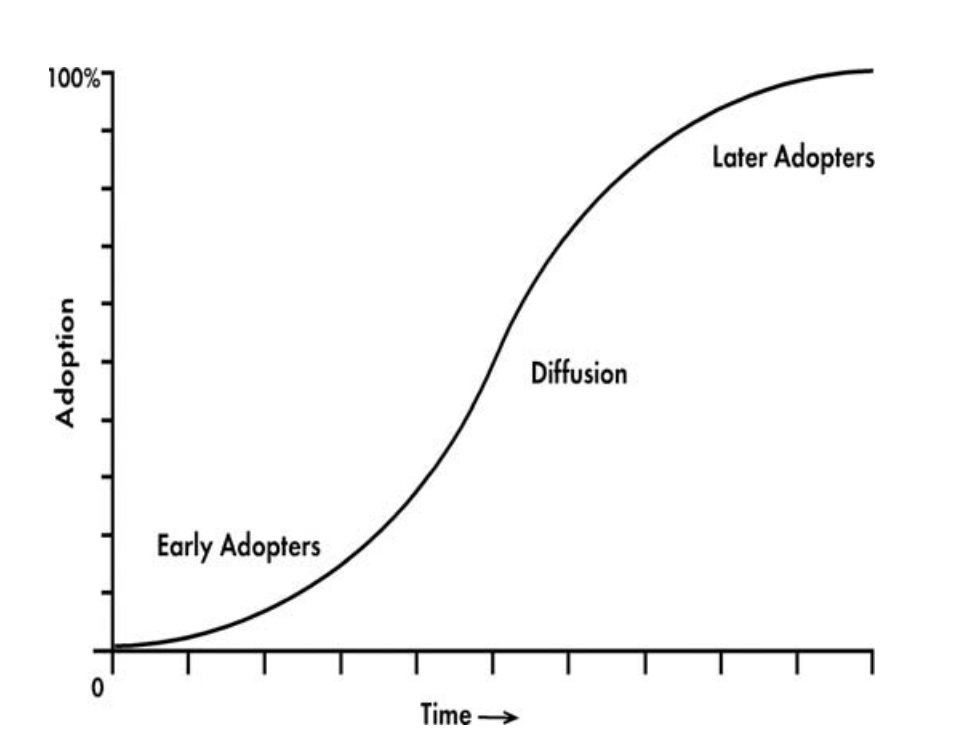
\includegraphics[scale=0.4]{scurve}
\caption[The S-curve]{The S-curve \cite{scurve}}
\label{fig:scurve}
\end{center}
\end{figure}
\begin{figure}
\begin{center}
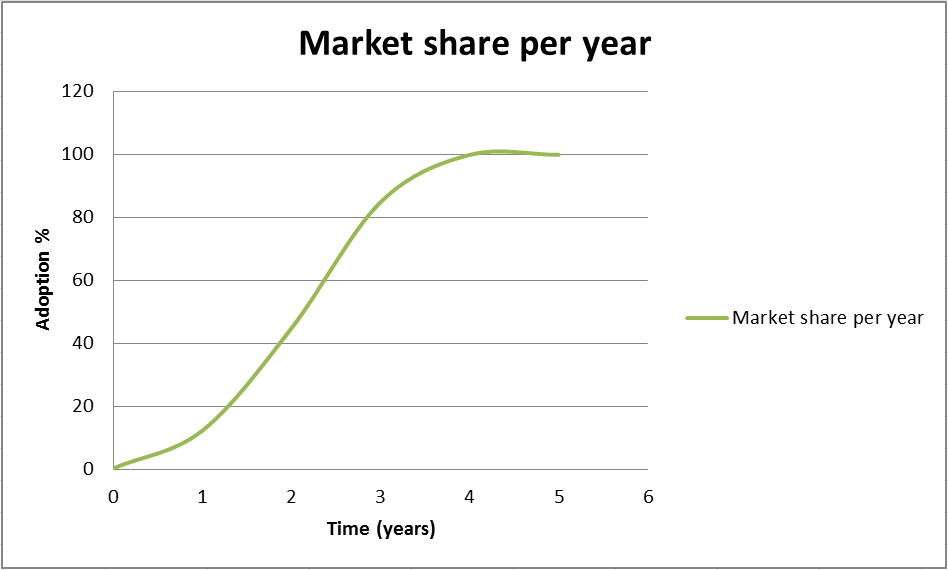
\includegraphics[scale=0.5]{scurve2}
\caption[The S-curve]{S-curve for the exergame. In this graph year 0 to 1 means the first year after the release.}
\label{fig:scurve2}
\end{center}
\end{figure}
\begin{figure}
\begin{center}
\includegraphics[scale=0.8]{revenuestreamprice}
\caption[Price example]{The lowest possible package price Cyberlab can have, provided that they sell the max amount of  copies - 1 200 units, is 2 700 NOK}
\label{fig:RevenueStreamPrice}
\end{center}
\end{figure}
\textbf{Pricing}\\ \\
The product price depends on existing games and tools, and Cyberlabs development costs. Estimating a suitable product price will be done by financial analysis and by looking at related, existing products on the market. Cyberlab's exergame falls under two definitions, a video game and a tool used in physiotherapy for training and rehabilitation. The video game market today exist of a huge amount of various games. They are mostly in an affordable price range, where e.g. Nintendo Wii games are priced between 99 - 499 NOK \cite{elkjopwii} and Xbox Kinect games are priced between 199 - 399 NOK \cite{elkjopkinect}. In addition there will be a cost of buying the needed hardware. Physiotherapy tools has more variation in price range as the definition of this tools are quite wide. Prices can vary from a fixed price of 120 NOK for a stretch pulley \cite{stretchpulley}, 11 000 NOK per month for shockwave therapy leasing (see Appendix C), up to 75 000 NOK for a treadmill \cite{treadmill}. Trying to sell the exergame for more than the already existing video games will be difficult, so it is therefore highly important for Cyberlab to promote their product as more than just a regular game to justify the price difference. This should be done by emphasizing the products value propositions, which relates the product more to physiotherapy equipment than "just" a video game. \\ \\
We will now present a detailed analysis for the two revenue models, and provide different price recommendations for the product. It is important to distinguish between Cyberlab's revenue and the package price presented for the customers. The product package shall as mentioned include the exergame and the Kinect sensor, but it is not the intention that Cyberlab shall make profit from reselling the Kinect sensors. The price a customer pays when buying a product package will balance Cyberlab's expense from purchasing a Kinect sensor, which makes it possible to neglect this cash flow from the analysis. Therefore, only software price will be taken into consideration in our analysis. A suitable price for the software should cover all expenses related to development, investment and marketing of the product. For simplicity, Cyberlab's total cost is rounded up to 3 240 000 NOK in our calculations. The price for the Kinect sensor is also rounded up to 2 000 NOK. \\ \\ 
\emph{Solution 1 - Fixed Price Model}\\ \\
As the exergame can be related to video games, a reasonable price would be a price similar to other video games on the market. The price range of existing Xbox Kinect games are 199 – 399, so we choose to price the game at 300 NOK. How Cyberlab’s revenue will develop with this price is shown in Figure \ref{fig:FixedLowPrice}. We observe that Cyberlab has to sell about 10 800 units to cover their total cost, which is an amount almost ten times higher than the potential market share of 1 200 physiotherapy clinics. We can therefore conclude that it will be impossible for Cyberlab to sell their game for a price as low as 300 NOK without experiencing huge economic loss.\\ \\
\begin{figure}
\begin{center}
\includegraphics[scale=0.7]{fixedlowprice}
\caption[Price related to commercial video games]{Total cost and revenue with price at 300 NOK. We observe that Cyberlab has to sell about 10 800 units to gain some profit}
\label{fig:FixedLowPrice}
\end{center}
\end{figure}
If we assume that Cyberlab has the possibility to sell their product to all of the 1 200 physiotherapy clinics in Norway, they could have a price as low as 2 700 NOK, see Figure \ref{fig:RevenueStreamPrice}, without gaining negative profit. However, it is as mentioned very risky, and almost unreasonable, to assume that Cyberlab could reach out to all potential target customers. \\ \\
Figure \ref{fig:RevenueStreamQuantity} shows three income lines related to three different prices, and how much Cyberlab, with each price, has to sell to cover their costs. With a price of 6 000 NOK Cyberlab needs to sell at least 540 units to achieve non-negative profit, but with a price of 10 000 NOK they only has to sell 324 units, see Table \ref{tab:unitsfixed}. Selling to the expected market share, Cyberlab can price 405 units at 8 000 NOK, which will balance Cyberlab's profit. Figure \ref{fig:RelationPriceAndUnits} shows every combination of price and quantity that will make a revenue of 3 240 000 NOK, which covers all of Cyberlab's costs related to developing this exergame. However, we believe that Cyberlab is interested in earning more then 0 NOK, so we recommend to sell the software for 10 000 NOK. To also include the Kinect sensor in the final package price, a customer will have to pay approximately 12 000 for the product package. We see that a fixed price package like this has a much higher price than existing video games on the market, however, it still is in the affordable area with regard to physiotherapy equipment. \\ \\
The sale of the product package will follow an earlier described s-curve, where the sale of the 400 units are distributed over the five year lifetime of the exergame. Table \ref{tab:revfixed} shows the expected revenue when selling 400 product packages. We observe that Cyberlab will gain a profit of 1 099 097 NOK by selling the product package at a fixed price of 12 000 NOK. Figure \ref{fig:ProfitFixed} shows the relationship between the accumulated revenue, costs and profit, with the fixed price model, over a five year period. From this figure we can see that Cyberlab will start to gain profit after about two and a half year. \\ \\
\begin{table}
\centering
    \begin{tabular}{|l|r|r|r|r|r|r|}
        \hline
       \textbf{Fixed price}  & & & & & \\ \hline
      \textbf{Price} & 300 & 2 700 & 6 000 & 8 000 & 10 000 \\ \hline
	   \textbf{Units to be sold} & 10 800 & 1 200 & 540 & 405 & 324 \\ \hline	
    \end{tabular}
    \caption[Price and Unit examples with the fixed price model]{Relation between package price and units to be sold to cover the total cost of 3 240 000. See appendix for calculations.}
    \label{tab:unitsfixed}
\end{table}

\begin{table}
\centering
    \begin{tabular}{|l|r|r|r|r|r|r|}
        \hline
       \textbf{Fixed price}  & & & & & & \\ \hline
      \textbf{Year} & \textbf{1} & \textbf{2} & \textbf{3} & \textbf{4} & \textbf{5} & \textbf{Total}\\ \hline
	   \textbf{Units sold} & 48 & 132 & 160 & 56 & 4 & \textbf{400}\\ \hline
	   \textbf{Revenue} & 576 000 & 1 584 000 & 1 920 000 & 672 000 & 48 000 & \textbf{4 800 000} \\ \hline  
	   \textbf{PV} & 553 846 & 1 464 497 & 1 706 873 & 574 824 & 39 453 & \textbf{4 339 097}  \\ \hline
    \end{tabular}
    \caption[Revenue with use of Fixed Price Model]{Revenue (in \ac{nok}) on a per year basis with the fixed price model. See appendix for calculations}
    \label{tab:revfixed}
\end{table}

\begin{figure}
\begin{center}
\includegraphics[scale=0.7]{revenuestreamquantity}
\caption[Quantity examples]{Total cost and three revenue lines related to three price examples; 6 000 NOK per unit, 8 000 NOK per unit and 10 000 NOK per unit, shows minimum number of units Cyberlab has to sell to achieve a non-negative profit}
\label{fig:RevenueStreamQuantity}
\end{center}
\end{figure}
\begin{figure}
\includegraphics[scale=0.6]{relationpriceandunits}
\caption[Relation between price per unit and number of sold units]{This figure shows every combination of unit price and number of sold units which will cover Cyberlab's total costs}
\label{fig:RelationPriceAndUnits}
\end{figure}
\begin{figure}
\begin{center}
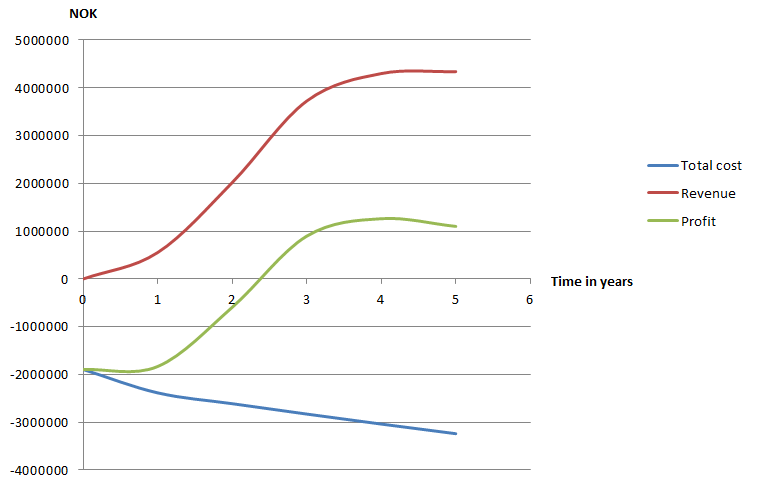
\includegraphics[scale=0.8]{profitfixed}
\caption[Profit, Revenue and Cost for a Fixed Price Solution]{This graph shows relation between costs, revenue and profit in a fixed price solution}
\label{fig:ProfitFixed}
\end{center}
\end{figure}
\emph{Solution 2 - Usage Fee Model}\\ \\
We will start by making an estimation of how much the exergame potentially will be used at physiotherapy clinics. Usually, a physiotherapist works approximately 8 hours each day, which includes 30 minutes lunch. Not every patient visiting the physiotherapy clinic during a regular day falls under the category “elderly”, and not every elderly visiting the clinic has the need for or wants to use this exergame. We roughly estimate that the exergame will be used approximately 2 hours each day. A physiotherapist works 47 weeks a year, assuming they have 5 weeks of vacation, and this adds up to 470 hours a year where the exergame will be used.\\ \\
Our first package price proposal in this usage fee model is a start price of 2 000 NOK for the package and a price of 10 NOK for each hour physiotherapists use the exergame. During a year this will add up to 4 700 NOK if the game is used as much as estimated. Here the Kinect sensor is included in the package price. Therefore, since Cyberlab’s revenue should be measured without consideration of the Kinect sensor, we subtract the Kinect sensor expense from the expected income. Each customer choosing the usage fee model will give Cyberlab an estimated revenue stream of approximately 2 700 NOK. For Cyberlab to be able to cover all costs they have to sell 1 200 packages. This means that they have to sell to all of the potential customers, which we have mentioned is quite unrealistic. We therefore provide another price proposal. We use the same startup price, but chose a price of 50 NOK for each hour the exergame is used. This will add up to 25 500 NOK, and without the Kinect sensor expenses Cyberlab has a revenue of approximately 23 500 NOK. In this case, Cyberlab only needs to sell 138 units to make a profit, a significant difference from the previous price example. \\ \\
To not experience severe economic loss by using this model, Cyberlab highly depends on their customers using the product. If no one uses the product after buying it, Cyberlab would not gain more revenue than from the startup price of 2 000 NOK per package. Figure \ref{fig:RevenueStreamUsage} shows that Cyberlab would have to sell 1 585 packages to gain profit if we do not take usage fee into consideration. This support the fact that Cyberlab is dependent on the exergame being used. \\ \\
As with the fixed price model we assume that Cyberlab is able to reach the realistic market share of 400 physiotherapy clinics. Table \ref{tab:revusage} shows Cyberlab's revenue when selling 400 units over a five year period. We assume that the exergame is used as much as estimated. To be able to calculate a revenue stream created by a sold package, we have looked at the start price and usage fees throughout one year as one total income. See appendix for details. We observe that the income increases much more in this usage fee example than in the fixed price example. Where we in the first example showed that Cyberlab barely achieved profit by selling 405 units, they can by this usage fee model sell 400 units to a profit of 5 257 399 NOK (See Appendix blabla). Figure \ref{fig:ProfitUsageFee} shows the relationship between the accumulated revenue, costs and profit, with the usage fee model, over a five year period. We observe that Cyberlab will gain profit after about one and a half year, one year earlier than with the fixed price model. \\ \\

\begin{figure}
\begin{center}
\includegraphics[scale=0.8]{revenuestreamusage}
\caption[Usage fee example - only sales]{Cyberlab depends on customer using the product. If no one use the product, Cyberlab has to sell 1 585 packages to gain profit}
\label{fig:RevenueStreamUsage}
\end{center}
\end{figure}
\begin{figure}
\begin{center}
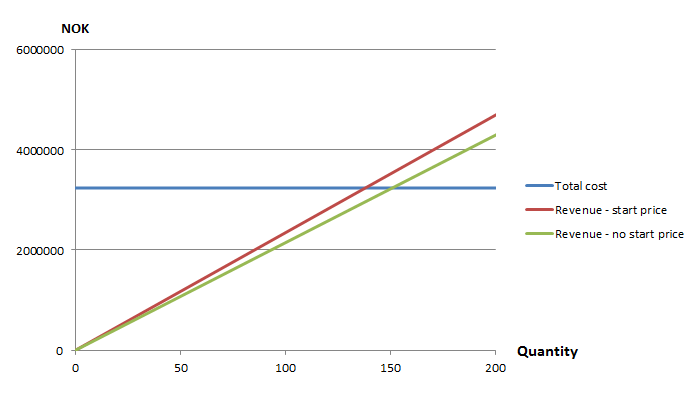
\includegraphics[scale=0.8]{usagewithwithoutstartprice}
\caption[Usage fee example]{Revenue with and without up-front price for the product package}
\label{fig:UsageWithWithout}
\end{center}
\end{figure}
Another solution for the usage fee model is for Cyberlab to give away their product package for free and just rely on the customers using the product. Figure \ref{fig:UsageWithWithout} shows the revenue streams when having an initial start price and when the product package is given away for free. We can see that there is not that much of a difference between these two examples. If Cyberlab give their product package away for free and customers use the exergame as much as we have estimated, they need to give away 151 packages    to gain profit. \\ \\

\begin{table}
    \begin{tabular}{|l|r|r|r|r|r|r|}
        \hline
       \textbf{Usage fee}  & & & & & & \\ \hline
      \textbf{Year} & \textbf{1} & \textbf{2} & \textbf{3} & \textbf{4} & \textbf{5} & \textbf{Total}\\ \hline
	   \textbf{Units sold} & 48 & 132 & 160 & 56 & 4 & \textbf{400}\\ \hline
	   \textbf{Revenue} & 1 128 000 & 3 102 000 & 3 760 000 & 1 316 000 & 94 000 & \textbf{9 400 000} \\ \hline  
	   \textbf{PV} & 1 084 615 & 2 867 973 & 3 342 626 & 1 124 922 & 77 261 & \textbf{8 497 399}  \\ \hline
    \end{tabular}
    \caption[Revenue with use of Usage Fee Model]{Revenue (in \ac{nok}) on a per year basis with the usage fee model. We have taken into consideration that the exergame will be used as estimated. For calculations, see appendix}
    \label{tab:revusage}
\end{table}
We can conclude that the best solution for Cyberlab will be to use the usage fee model. There is a high risk related to profit, but the profit has the potential of becoming much higher than with a fixed price model. As mentioned, the low startup price for the usage fee model is not alone enough to cover all of Cyberlabs costs, so even if Cyberlab manage to cover the whole market they will experience a economic loss if no one use the product. If we predict that Cyberlab sell the likely amount of 400 units, but the product never get used, they will not gain any revenue at all. This is because the income of 2 000 NOK per package will be used to cover the Kinect sensor expenses. Cyberlab will therefore have a negative profit equal to the total costs. The loss will become even bigger if Cyberlab chooses the usage fee model that includes giving the product package away. However, in both cases, if all of the 400 customers use the exergame only one hour each day for a year, it will be enough for Cyberlab to gain non-negative profit. Also, if there are only one exergame at a physiotherapy clinic, the game would be shared among several physiotherapists, and we can expect the exergame to be used more. Expected life time for the exergame is approximately five years, so Cyberlab is actually only dependent on customers using the game one hour a week, which is very likely. \\ \\   
So, which pricing mechanism should Cyberlab use in the usage fee model? When selling 400 units, there is a difference in profit of 800 000 NOK in choosing the model with startup price of 2 000 NOK instead of the give-away solution. From a customers point of view there will be very attractive to get this product package for free. A possible drawback with the give-away solution is that customers do not have the same incentive to use a product they get for free as they have with a product they have paid for. With a free product package they have nothing to lose by not using it. Because of this, and the risk already related to the usage fee model, we recommend Cyberlab to chose the startup price solution. \\ \\ 
For the customers point of view a usage fee model will appear more appealing than a fixed package price because of the low startup price. Customers observe that the product price is higher than other existing video games on the market, but they also know what value propositions this exergame holds, which justify the price difference. They also have information about prices on equipment used at physiotherapy clinics, which makes Cyberlab’s usage fee model affordable. Customers also have other reasons for why they prefer this solution. One example is “Ilen Fysioterapi og Idrett”, a private physiotherapy clinic with no economic support from the government, which sees a security in the possibility of buying the product with a usage fee model (Se Appendix C). The startup price is manageable, and they can control additional costs themselves after how much they want to use the equipment. Private physiotherapists might not have the same financial resources as local institutes, so the idea of paying according to how much they use the product is appealing.  \\ \\
Figure \ref{fig:RevenueAll} presents six revenue streams examples from both the fixed price model and the usage fee model. We have included three different fixed prices, two different usage fees, and usage fee with and without start price. We still estimate that Cyberlab is able to sell 400 units, and that the game, with the usage fee model, is used as much as estimated. The revenue streams is presented on a per year basis, during a life time of five years. Number of units sold per year is distributed by the s-curve. We clearly see that the solution with a usage fee model, with start price and fees at 50 NOK, gives the highest revenue.  
\begin{figure}
\begin{center}
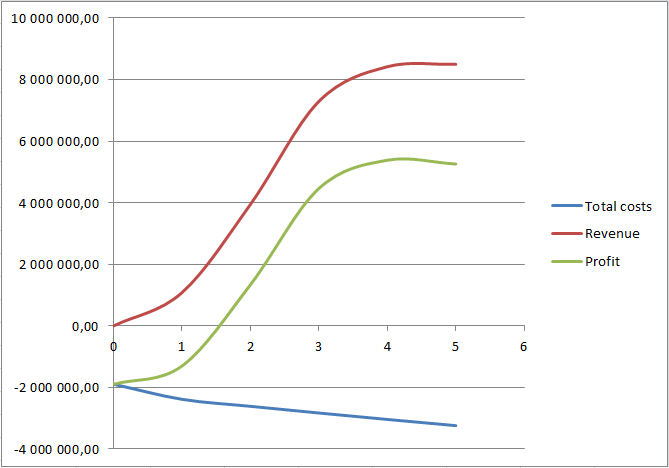
\includegraphics[scale=0.8]{profitusagefee}
\caption[Profit, Revenue and Cost for a Usage Fee Solution]{This graph shows relation between costs, revenue and profit in a usage fee solution with startup price}
\label{fig:ProfitUsageFee}
\end{center}
\end{figure}

\begin{figure}
\begin{center}
\includegraphics[angle=90,scale=0.5]{revenueall}
\caption[Revenue examples for both fixed price model and usage fee model]{This graph represents several revenue examples for both the fixed price and usage fee. Revenue is represented on a per year basis. See appendix for calculations.}
\label{fig:RevenueAll}
\end{center}
\end{figure}


Må skrive litt om grafene som viser per år her